\documentclass[10pt]{article}
\usepackage[margin=0.75in]{geometry}
\usepackage{graphicx}
\usepackage{booktabs}
\usepackage{hyperref}
\usepackage[T1]{fontenc}
\title{Weak-curve evidence database: exact classes, diagnostics and construction}
\author{Research report}
\date{12 October 2026 UTC}
\begin{document}
\maketitle
\noindent\textbf{Contribution.}
The fixed public research corpus is now a queryable SQLite database with
339,740 class observations, 814 exact models, 21 family or condition entries
with a proof obligation for each,
12 construction recipes, ten theorem records, four heuristic records and
eight hypothesis entries. The cubic norm-one identity and fourth-power
corollary have six checked Lean declarations. The import preserves model, class, covering and
selected-subgroup evidence as separate claims.

\begin{center}
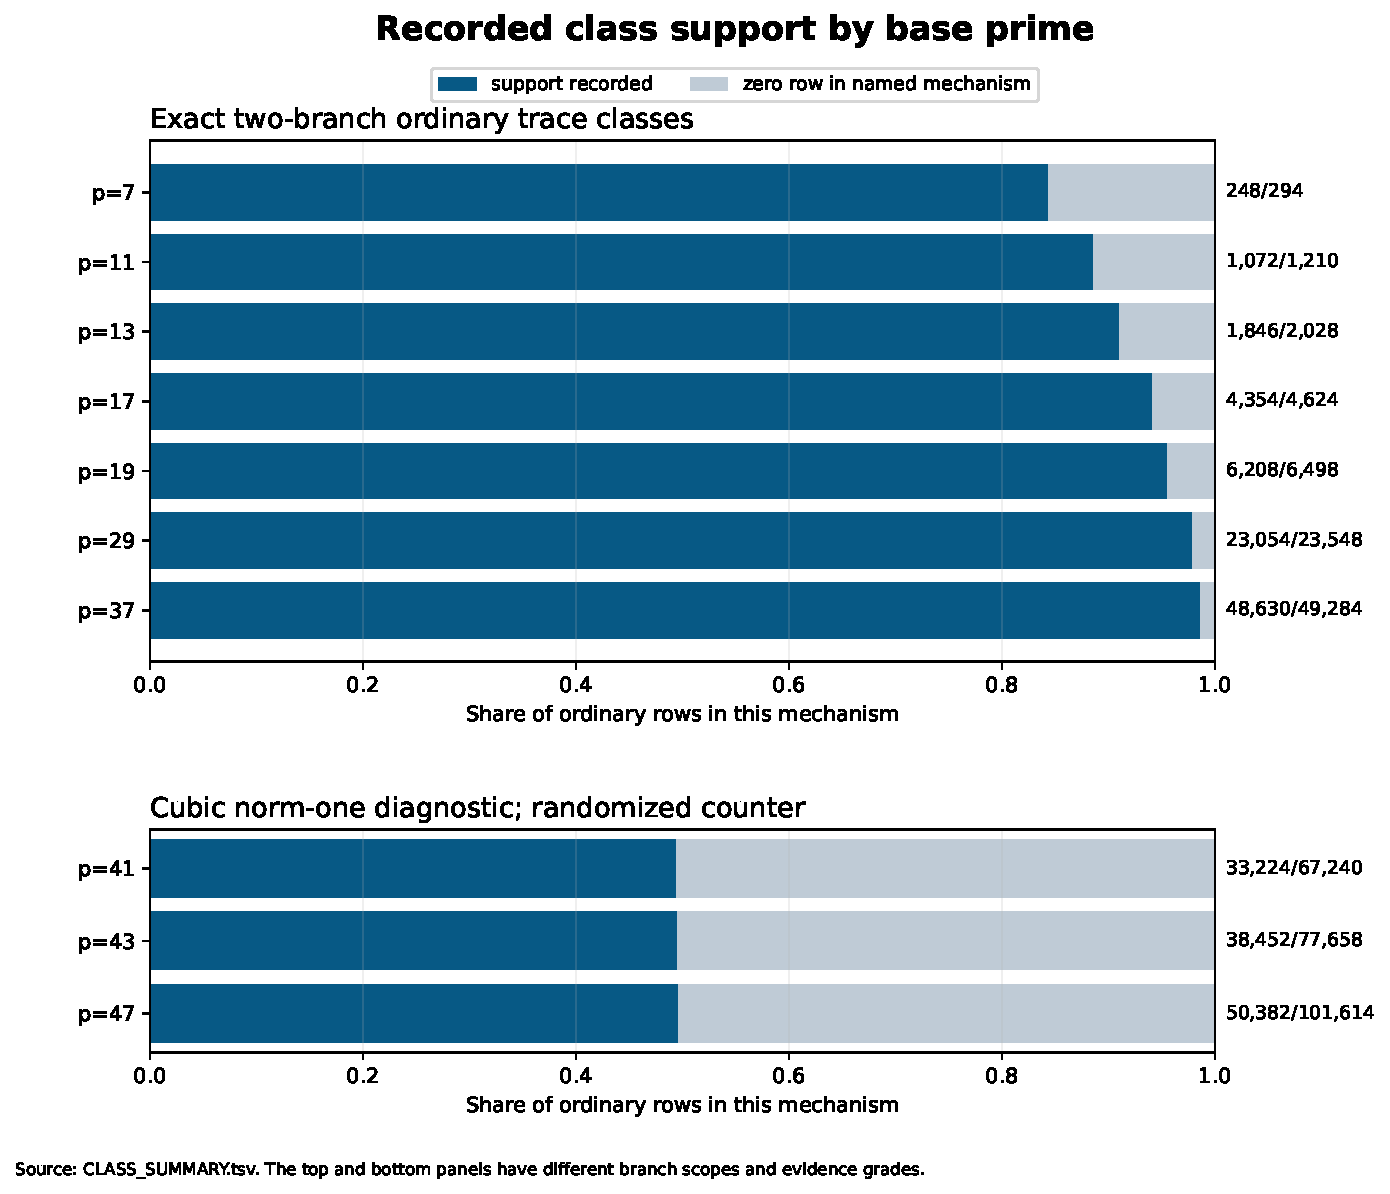
\includegraphics[width=\linewidth,height=0.54\textheight,keepaspectratio]{class_counts_plot.pdf}
\end{center}

\noindent The upper panel contains 87,486 complete exact ordinary rows for
the two named hyperelliptic genus-three branches at
$p=7,11,13,17,19,29,37$: 85,412 union-positive and 2,074 union-zero.
The lower panel imports 252,254 Hasse candidates at $p=41,43,47$
for the earlier cubic norm-one census; 246,512 are ordinary.
Those latter rows used randomized point counting, so zero labels remain
diagnostic. The scopes and grades are never combined as a prevalence law.

\newpage
\section*{Construction theorem and route}
Let $L=\mathbf F_{q^3}$ with $q=p^2$ and $p>3$. For nonzero $\alpha$,
put $\lambda=\alpha^q/\alpha$. The conjugate ratios telescope:
\[
\lambda\lambda^q\lambda^{q^2}
=\frac{\alpha^q}{\alpha}
 \frac{\alpha^{q^2}}{\alpha^q}
 \frac{\alpha^{q^3}}{\alpha^{q^2}}=1.
\]
Thus $\lambda^{q^2+q+1}=1$. Since $q^2+q+1$ is odd, this parameter
is a fourth power in its torus. The cubic covering route forms
$E:y^2=x(x-\alpha)(x-\alpha^q)$, then verifies the smooth
genus-three cover and its map to the full Weil restriction.
The prior ISO-1 theorem gives the necessary ordinary conductor screen
$v_2(f_\pi)\geq2$ for both twist signs. Exact class support uses its
selected CM-order intersection or exceptional finite oracle.

\medskip\noindent The new Lean declarations prove the norm identity in a
commutative multiplicative group under a cubic automorphism, and the
exponent conclusion under the explicit hypothesis
$\sigma(x)=x^q$. For odd $p$ and $q=p^2$, they also construct the
fourth root $\lambda^{(q^2+q+2)/4}$ from the exact torus exponent
equation. They do not assume norm one. Full elliptic-curve
covering, isogeny, selected-subgroup and CM bridges remain separate
obligations with their exact status in \texttt{PROOF\_MAP.md}. The
denominator-cleared polynomial identity has native certificate
\texttt{IDC1h3561e7fee541a297}.

\section*{Evidence contract}
The native importer checks all 19 source hashes, full trace domains,
branch-union flags, exact model identities, point-count arithmetic and
814 model/property links. Reimported table contents, TSV and SVG match.
The model inventory includes 537 identities over 192--252-bit fields:
384 remain unclassified by this covering-model index and 153 are outside
its stated domain. Selected-subgroup advantage is unmeasured for these
537 records. At 17 bits, 24 exact models have a positive cubic or
quadratic covering-model label.
The new Lean module builds and its six public roots have only
propext and Quot.sound in their transitive axiom lists.

\begin{center}
\begin{tabular}{@{}p{0.27\linewidth}p{0.63\linewidth}@{}}
\toprule
Record & Meaning and present status\\
\midrule
Exact class row & Certified two-branch ordinary trace label on the stated finite domain.\\
Diagnostic row & Earlier cubic norm-one representative count; zero labels depend on randomized counting.\\
Model row & Exact field and Weierstrass model; an ICV1 key and source hash bind its properties.\\
Mechanism row & Construction and witness checklist; a selected subgroup needs its own map and cost evidence.\\
\bottomrule
\end{tabular}
\end{center}

\section*{Next import}
The published Iijima--Momose--Chao Type I/II classification is the
first table-level import. Its 17 additional cases span source genera
beyond elliptic curves, so equations, twists, fields and equivalence
relations must be normalized before adding records. Tian's odd-prime
polarized cubic-restriction construction is a separate mechanism
backlog. A prospective complete two-branch census follows with
frozen input and independent validation. Full source links and
receipts are in \texttt{REPORT.md}, \texttt{SOURCE\_AUDIT.md} and
\texttt{VALIDATION.md}.
\end{document}
